\documentclass[border=3pt]{standalone}
\usepackage{tikz}
\usetikzlibrary{arrows.meta,calc,positioning}
\tikzset{pin/.style={-{Stealth[length=5pt]}},
  ff/.style={draw, thick, minimum width=11mm, minimum height=15mm, font=\sffamily\small}}
\begin{document}
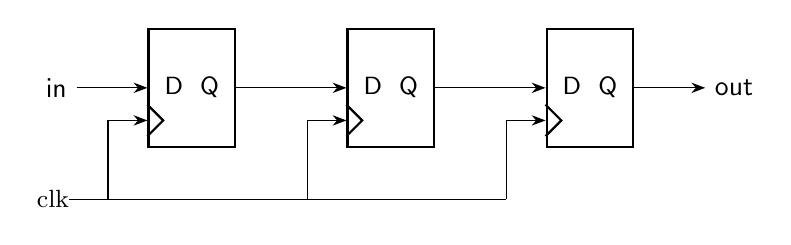
\begin{tikzpicture}[font=\sffamily, node distance=14mm]
  \node[ff] (f0) {D\ \ Q};
  \node[ff, right=of f0] (f1) {D\ \ Q};
  \node[ff, right=of f1] (f2) {D\ \ Q};
  % clock-input coordinate for each FF (wedge centre on the west edge, low, clear of D)
  \foreach \n in {f0,f1,f2}{\coordinate (\n c) at ($(\n.south west)+(0,3.5mm)$);
    \draw[thick] ($(\n.south west)+(0,1.5mm)$) -- ++(2mm,2mm) -- ++(-2mm,2mm);}
  \draw[pin] ($(f0.west)+(-9mm,0)$) node[left]{in} -- (f0.west);
  \draw[pin] (f0.east) -- (f1.west);
  \draw[pin] (f1.east) -- (f2.west);
  \draw[pin] (f2.east) -- ++(9mm,0) node[right]{out};
  % shared clk rail below the FF row; branches rise and enter the west edge
  \coordinate (c0) at ($(f0c)+(-5mm,-10mm)$);
  \coordinate (c2) at ($(f2c)+(-5mm,-10mm)$);
  \node[font=\small] at ($(c0)+(-7mm,0)$){clk};
  \draw ($(c0)+(-5mm,0)$) -- (c2);
  \draw[pin] (c0) |- (f0c);
  \draw[pin] ($(f1c)+(-5mm,-10mm)$) |- (f1c);
  \draw[pin] (c2) |- (f2c);
\end{tikzpicture}
\end{document}
